\input{mmd-beamer-header-11pt}
\def\mytitle{Part 2: Frequentist statistical building blocks}
\def\mydate{25 March 2015}
\def\myauthor{Matthew Pitkin}
\def\affiliation{University of Glasgow}
\def\latexxslt{beamer}
\def\latexmode{beamer}
\def\theme{m}
\def\event{GraWIToN School}
\input{mmd-beamer-begin-doc}


% Part 2 of my lecture course on statistics for the GraWIToN school
%
% Frequentist statistical building blocks


\begin{frame}

\frametitle{Overview}
\label{overview}

In this part of the course we will discuss

\begin{itemize}
\item parameter estimation

\item maximum likelihood

\item hypothesis testing

\item goodness-of-fit

\end{itemize}

from a Frequentist perspective.

\end{frame}

\begin{frame}

\frametitle{The sampling distribution}
\label{thesamplingdistribution}

Suppose we observe $n$ different realisations of a variable $x$ (e.g. the height of everyone in the class),
which has a pdf $p(x|I)$ (e.g. a normal distribution). This set
$\{x_1,\ldots,x_n\}$ is called a \textbf{random sample from the population with pdf} $p(x|I)$.
The joint pdf of these samples, $g(x_1,\ldots,x_n)$, is known as the \textbf{sampling distribution}. If all
the elements, $x_i$, are \textbf{independently and identically distributed} (iid) then
\[
g(x_1,\ldots,x_n|I) = p(x_1|I)p(x_2|I)\ldots p(x_n|I)
\]
The sampling distribution is more commonly encountered as the \textbf{likelihood function}, which we will
discuss more later, and a \emph{random sample} will be considered to be some observed data set.

\end{frame}

\begin{frame}

\frametitle{Parameter estimation: statistics and estimators}
\label{parameterestimation:statisticsandestimators}

We may wish to study a population which has (or is assumed to have) a pdf $p(x|\theta,I)$, where $|$
indicates that the pdf is dependent some (possibly unknown) parameter $\theta$\footnote{In frequentist terms the pdf $p(x|\theta,I)$ would really be expressed as $p(x;\theta)$,
where $x$ is the RV dependent on the particular true value of $\theta$, which is therefore not a RV. In the
Bayesian view both $x$ and $\theta$ have associated pdfs, so our knowledge of
$\theta$ is just given by its pdf and any particular value range just has an associated plausibility.}.

If we observe a random sample from the population $\{x_1,\ldots,x_n\}$ we might want to try and use these
to estimate $\theta$. How can we do that?

\end{frame}

\begin{frame}

\frametitle{Parameter estimation: statistics and estimators}
\label{parameterestimation:statisticsandestimators}

A \textbf{statistic} is a function of observable RVs that \emph{does not} depend on any unknown parameters.
For a random sample drawn from $p(x|\theta,I)$ any function of $\{x_1,\ldots,x_n\}$ that \emph{does not}
depend on $\theta$ is an example of a statistic.

E.g., if a value $x_1$ is drawn from a normal distribution, $p(x|\mu,\sigma,I)$, where $\mu$ and $\sigma$ are not
known \emph{a priori} then $x_1-\mu$ is \textbf{not} a statistic.

However, in frequentist parameter estimation the idea is to use \emph{statistics} to estimate the unknown parameters
of a pdf\footnote{In the Bayesian view you would just calculate the pdf of the unknown parameters.}.

\end{frame}

\begin{frame}

\frametitle{Parameter estimation: statistics and estimators}
\label{parameterestimation:statisticsandestimators}

An \textbf{estimator} (e.g. $\hat{\theta}$) is a statistic used to estimate the value of a parameter (e.g. $\theta$).
$\hat{\theta}$ is not a funciton of $\theta$, but is itself a RV as it is just a function of RVs $\{x_1,\ldots,x_n\}$.

Since $x$ depends on the \emph{true} value of $\theta$ then so does pdf of $\hat{\theta}$ and also $p(\hat{\theta}|\theta)$.
The distribution $p(\hat{\theta}|\theta)$ can be determined by repeated trials (observations\slash experiments) giving new
\textbf{random samples}, and the properties of $p(\hat{\theta}|\theta)$ can be used to determine if $\hat{\theta}$ is
a \emph{``good''} estimator of the \emph{true} $\theta$.

\end{frame}

\begin{frame}

\frametitle{Parameter estimation: statistics and estimators}
\label{parameterestimation:statisticsandestimators}

\begin{columns}
\begin{column}{0.55\textwidth}

The pdfs of two estimators of $\theta$ ($\hat{\theta}_1$ and $\hat{\theta}_2$) are shown.

\begin{itemize}
\item $p(\hat{\theta}_1|\theta,I)$ is broad and carries a large \textbf{statistical error}, but does encompass the true value of $\theta$

\item $p(\hat{\theta}_2|\theta,I)$ is narrow, but offset from the $\theta$, and can be said to have large \textbf{systematic errors}

\end{itemize}

It can be difficult to decide which estimator is \emph{``best''} (especially when the true value is unknown).

\end{column}
\begin{column}{0.45\textwidth}

\begin{figure}[htbp]
\centering
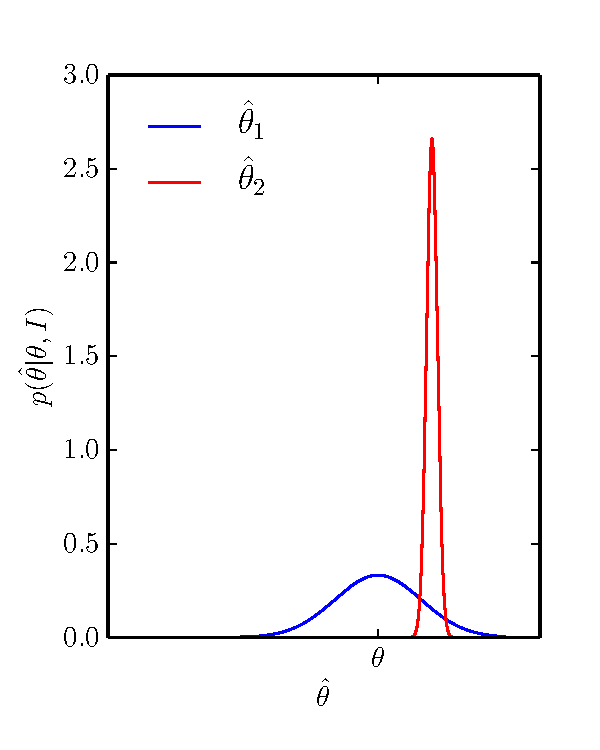
\includegraphics[keepaspectratio,width=\textwidth,height=250pt]{figures/estimator.pdf}
\label{estimator}
\end{figure}

\end{column}
\end{columns}

\end{frame}

\begin{frame}

\frametitle{Parameter estimation: statistics and estimators}
\label{parameterestimation:statisticsandestimators}

\begin{columns}
\begin{column}{0.55\textwidth}

\begin{itemize}
\item $\hat{\theta}_1$ is an \textbf{unbiased} estimator

\begin{itemize}
\item repeated observations would average to the true value, e.g. $E[\hat{\theta}_1] = \int \hat{\theta}_1 p(\hat{\theta}_1|\theta,I) {\rm d}\hat{\theta}_1 = \theta$.

\item \emph{but} $\text{var}[\hat{\theta}_1]$ is large

\end{itemize}

\item $\hat{\theta}_2$ is a \textbf{biased} estimator

\begin{itemize}
\item $E[\hat{\theta}_1] = \int \hat{\theta}_2 p(\hat{\theta}_2|\theta,I) {\rm d}\hat{\theta}_2 \ne \theta$.

\item \emph{but} $\text{var}[\hat{\theta}_2]$ is small

\end{itemize}

\end{itemize}

\emph{If} we could correct for bias $\hat{\theta}_2$ would be a better choice of estimator.

\end{column}
\begin{column}{0.45\textwidth}

\begin{figure}[htbp]
\centering
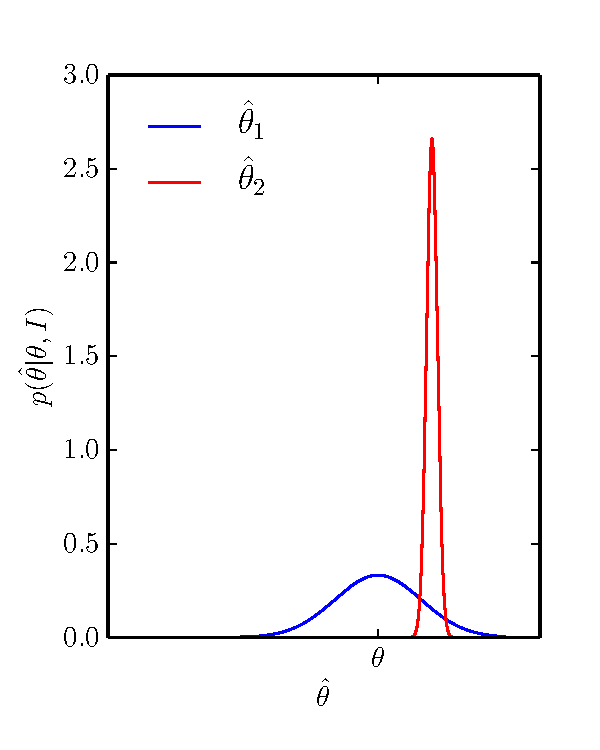
\includegraphics[keepaspectratio,width=\textwidth,height=250pt]{figures/estimator.pdf}
\label{estimator}
\end{figure}

\end{column}
\end{columns}

\end{frame}

\begin{frame}

\frametitle{Parameter estimation: the sample mean}
\label{parameterestimation:thesamplemean}

The simplest unbiased estimator is the \textbf{sample mean}. If we have a random sample $\{x_1,\ldots,x_n\}$ of length
$n$ drawn from pdf $p(x|I)$, which has unknown mean $\mu$ and variance $\sigma^2$, then
\[
\text{sample mean}=\hat{\mu} = \frac{1}{n}\sum_{i=1}^n x_i.
\]
This is an unbiased estimator of $\mu$ in that $E[\hat{\mu}] = \mu$.

The variance, $\sigma_{\hat{\mu}}^2$, of the sample mean (i.e. the width of the distribution $p(\hat{\mu}|\mu,I)$)
is
\[
\sigma_{\hat{\mu}}^2 = \sigma^2/n,
\]
so as the sample size increases the sample mean distribution becomes more concentrated around the
true mean (the \emph{law of large numbers}).

\end{frame}

\begin{frame}

\frametitle{Parameter estimation: the sample variance}
\label{parameterestimation:thesamplevariance}

If $\mu$ is known then an estimator for the variance is
\[
\hat{\sigma}^2 = \frac{1}{n}\sum_{i=1}^n (x_i-\mu)^2.
\]
and $E[\hat{\sigma}^2] = \sigma^2$ (i.e. it is \emph{unbiased}).

However, if $\mu$ is unknown and we instead use $\hat{\mu}$ in its place then
\[
E[\hat{\sigma}^2] = \frac{n-1}{n}\sigma^2,
\]
so it is \emph{biased}. In this case an \emph{unbiased} estimator of the \textbf{sample variance} is
\[
\hat{\sigma}^2 = \frac{1}{n-1}\sum_{i=1}^n (x_i-\hat{\mu})^2.
\]

\end{frame}

\begin{frame}

\frametitle{Parameter estimation: linear correlation}
\label{parameterestimation:linearcorrelation}

Given sampled data $\{(x_i, y_i); i=1,\ldots,n\}$ we can \emph{estimate} the linear correlation between the
variables as
\[
r = \frac{1}{n-1}\sum_{i=1}^n\Bigg(\frac{x_i-\redob{\hat{\mu}_x}^{\mathclap{\text{sample mean}}}}{\hat{\sigma_x}}\Bigg)
\Bigg(\frac{y_i-\hat{\mu}_y}{\hat{\sigma_y}}\Bigg)
\]
where, e.g.,
\[
\hat{\sigma}_x = \sqrt{\frac{1}{n-1}\sum_{i=1}^n (x_i-\hat{\mu}_x)^2 }.
\]
If $p(x,y|I)$ is a bivariate normal distribution then $r$ is an \textbf{estimator} is the correlation coefficient $\rho$.

\end{frame}

\begin{frame}

\frametitle{Parameter estimation: central limit theorem}
\label{parameterestimation:centrallimittheorem}

\begin{columns}
\begin{column}{0.25\textwidth}

For \emph{any} pdf with finite variance, $\sigma^2$, and mean, $\mu$, central limit theorem states that as
$n \rightarrow \infty$ the sample mean $\hat{\mu}$ has a normal pdf with
mean $\mu$ and variance $\sigma^2/n$.
\end{column}
\begin{column}{0.75\textwidth}
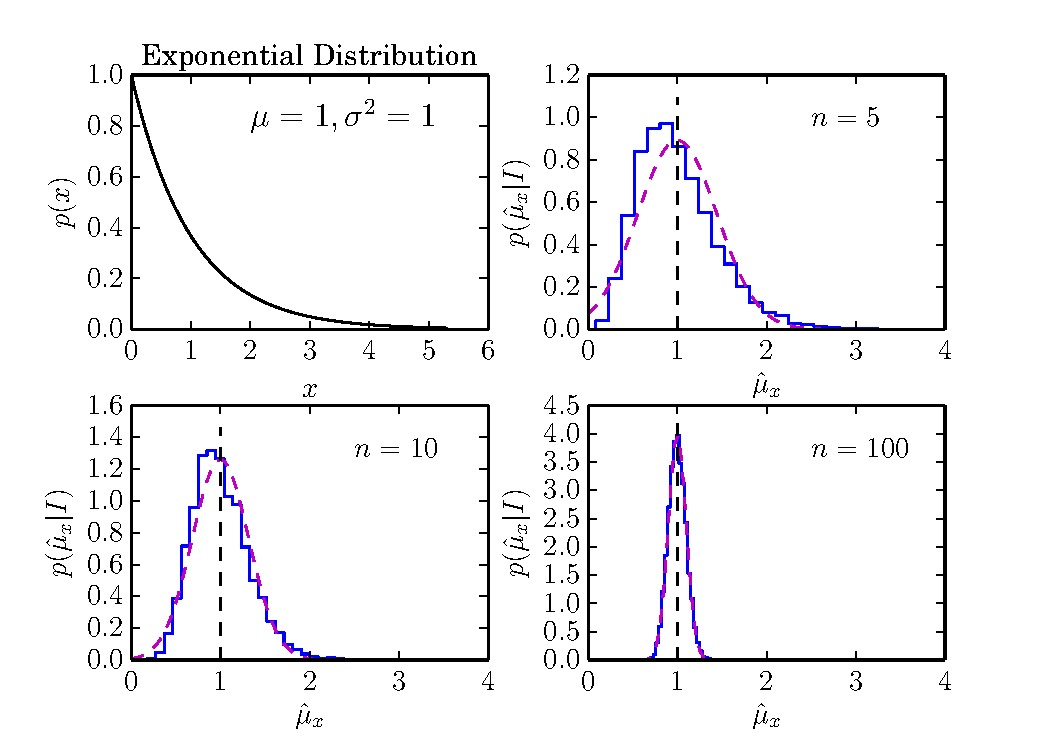
\includegraphics[keepaspectratio,width=\textwidth,height=250pt]{figures/central_limit_theorem.pdf}
\end{column}
\end{columns}

\end{frame}

\begin{frame}

\frametitle{Parameter estimation: least squares}
\label{parameterestimation:leastsquares}

\begin{columns}
\begin{column}{0.45\textwidth}

The method of \textbf{least squares} (LS) is a \emph{standard} (often ``black box'') method for fitting lines and
curves to data.

E.g. if we have some $\{x, y\}$ data least squares provides a way to find the \emph{``best fit''}
straight line $y = mx+c$ for it (i.e. estimates of the
values of the parameters $m$ and $c$ that minimise the sum of the squared residuals).
\end{column}
\begin{column}{0.55\textwidth}

\begin{figure}[htbp]
\centering
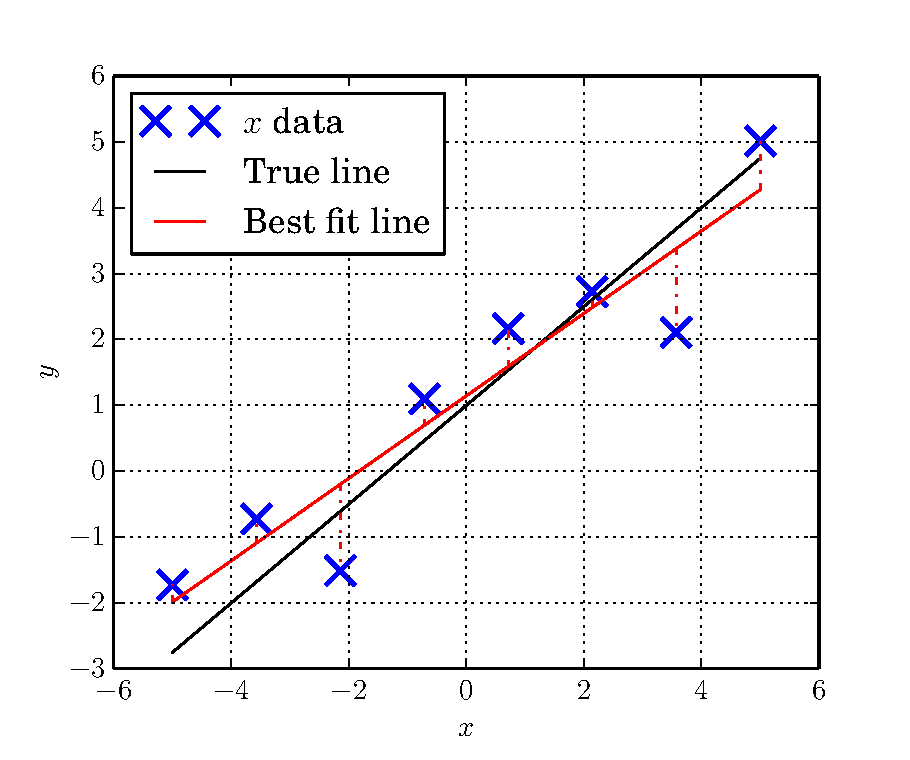
\includegraphics[keepaspectratio,width=\textwidth,height=210pt]{figures/linear_data.pdf}
\label{linear_data}
\end{figure}

\end{column}
\end{columns}

\end{frame}

\begin{frame}

\frametitle{Parameter estimation: ordinary linear LS}
\label{parameterestimation:ordinarylinearls}

\textbf{Ordinary linear least squares} assumes scatter in a plot of $\{x_i,y_i\}$ arises from errors in only one
of the two variables. We call the variable with (say $y$) and without (say $x$) error the
\textbf{dependent variable} and \textbf{independent variable} respectitvely. For each data point suppose we can write
\[
y_i = mx_i + c + \epsilon_i 
\]
where $\epsilon_i$ is known as the \textbf{residual} of the $i^{\rm th}$ data point, i.e. the difference
between the observed value $y_i$ and the value predicted by the best-fit straight line.

\end{frame}

\begin{frame}

\frametitle{Parameter estimation: ordinary linear LS}
\label{parameterestimation:ordinarylinearls}

We assume that the $\{\epsilon_i\}$ are an \emph{iid} random sample from some underlying pdf with
$\mu=0$ and variance $\sigma^2$.

The \textbf{least squares estimators} of $m$ and $c$ minimise the function
\[
S = \chi^2(m,c) = \redub{\sum_{i=1}^n \left(y_i - (mx_i + c)\right)^2}_{\mathclap{\sum_{i=1}^n \epsilon_i^2}}
\]
so $\hat{m}_{\rm LS}$ and $\hat{c}_{\rm LS}$ satisfy
\[
\left|\frac{\partial S}{\partial m}\right|_{m=\hat{m}_{\rm LS}} = 0 \text{ and } \left|\frac{\partial S}{\partial c}\right|_{c=\hat{c}_{\rm LS}} = 0
\]

\end{frame}

\begin{frame}

\frametitle{Parameter estimation: ordinary linear LS}
\label{parameterestimation:ordinarylinearls}

Solving these equations for the estimators we have:
\[
\hat{m}_{\rm LS} = \frac{n\sum y_ix_i - \sum y_i \sum x_i}{n\sum x_i^2 - \left(\sum x_i\right)^2}
\]
and
\[
\hat{c}_{\rm LS} = \frac{\sum y_i \sum x_i^2 - \sum y_ix_i \sum x_i}{n\sum x_i^2 - \left(\sum x_i\right)^2}.
\]
We can see these estimators \emph{are} statistics as they just depend on the data and not the $m$ and $c$ parameters,
or the (potentially unknown) variance of the residuals $\sigma^2$.

In can also be shown that these least squares estimators are \textbf{unbiased}, i.e. $E[\hat{m}_{\rm LS}] = m$ and
$E[\hat{c}_{\rm LS}] = c$.

\end{frame}

\begin{frame}

\frametitle{Parameter estimation: ordinary linear LS}
\label{parameterestimation:ordinarylinearls}

Assuming a \emph{known} variance on the residuals the variance of the estimators are
\[
\begin{array}{cl}
\text{var}[\hat{m}_{\rm LS}] &= \frac{\sigma^2n}{n\sum x_i^2 - \left(\sum x_i\right)^2} \\ 
\text{var}[\hat{c}_{\rm LS}] &= \frac{\sigma^2\sum x_i^2}{n\sum x_i^2 - \left(\sum x_i\right)^2}
\end{array}
\]
In general $\hat{m}_{\rm LS}$ and $\hat{c}_{\rm LS}$ will not be statistically independent, so they
have a covariance given by
\[
\text{cov}[\hat{m}_{\rm LS}, \hat{c}_{\rm LS}] = \frac{-\sigma^2\sum x_i}{n\sum x_i^2 - \left(\sum x_i\right)^2}
\]
We can see that if $\sum x_i=0$ (which, provided uniform sampling in $x$, we could always transform into) the estimators are uncorrelated.

\end{frame}

\begin{frame}

\frametitle{Parameter estimation: weighted linear LS}
\label{parameterestimation:weightedlinearls}

If the residuals $\{\epsilon_i\}$ are drawn from pdfs with $\mu=0$, but different \emph{known}
variances $\sigma_i^2$, then
\[
S = \chi^2(m,c) = \sum_{i=1}^n \left[\frac{y_i - (mx_i + c)}{\sigma_i}\right]^2
\]
We can find the \textbf{weighted least squares} estimators by again finding the solutions
that minimise $S$, giving
\[
\hat{m}_{\rm LS} = \frac{\sum\frac{1}{\sigma_i^2}\sum \frac{y_ix_i}{\sigma_i^2} - \sum \frac{y_i}{\sigma_i^2} \sum \frac{x_i}{\sigma_i^2}}{\sum\frac{1}{\sigma_i^2}\sum \frac{x_i^2}{\sigma_i^2} - \left(\sum \frac{x_i}{\sigma_i^2}\right)^2}
\]
and
\[
\hat{c}_{\rm LS} = \frac{\sum \frac{y_i}{\sigma_i^2} \sum \frac{x_i^2}{\sigma_i^2} - \sum \frac{y_ix_i}{\sigma_i^2} \sum \frac{x_i}{\sigma_i^2}}{\sum\frac{1}{\sigma_i^2}\sum \frac{x_i^2}{\sigma_i^2} - \left(\sum \frac{x_i}{\sigma_i^2}\right)^2}.
\]

\end{frame}

\begin{frame}

\frametitle{Parameter estimation: weighted linear LS}
\label{parameterestimation:weightedlinearls}

This also gives variances and a covariance of
\[
\text{var}[\hat{m}_{\rm LS}] = \frac{\sum \frac{1}{\sigma_i^2}}{\sum \frac{1}{\sigma_i^2}\sum \frac{x_i^2}{\sigma_i^2} - \left(\frac{x_i}{\sigma_i^2}\right)^2},
\]
\[
\text{var}[\hat{c}_{\rm LS}] = \frac{\sum \frac{x_i^2}{\sigma_i^2}}{\sum \frac{1}{\sigma_i^2}\sum \frac{x_i^2}{\sigma_i^2} - \left(\frac{x_i}{\sigma_i^2}\right)^2},
\]
and
\[
\text{cov}[\hat{m}_{\rm LS},\hat{c}_{\rm LS}] = \frac{-\sum \frac{x_i}{\sigma_i^2}}{\sum \frac{1}{\sigma_i^2}\sum \frac{x_i^2}{\sigma_i^2} - \left(\frac{x_i}{\sigma_i^2}\right)^2}
\]
If $\sigma_i^2$ is constant these all reduce to the unweighted case.

\end{frame}

\begin{frame}

\frametitle{Parameter estimation: LS generalisations}
\label{parameterestimation:lsgeneralisations}

What about errors on \emph{both} variables? The $\chi^2$ function to minimise becomes
\[
\chi^2(m, c) = \sum_{i=1}^n \frac{(y_i - mx_i - c)^2}{\sigma_{y,i}^2 + m^2\sigma_{x,i}^2}.
\]
The equations to minimise this are \emph{non-linear}, so these is no simple analytic solution. They must
be solved using numerical methods instead.

\end{frame}

\begin{frame}

\frametitle{Parameter estimation: LS generalisations}
\label{parameterestimation:lsgeneralisations}

We can generalise the linear model, e.g. to an $(M-1)^{\rm th}$ order polynomial
\[
y(x) = a_1 + a_2x + a_3x^2 + \ldots + a_Mx^{M-1} = \sum_{k=1}^M a_k x^{k-1}
\]
or even more generally $y(x) = \sum_{k=1}^M a_k X_k(x_i)$, where $X(x)$ is some function of $x$
multiplied by a coefficient, $a$, that we want an estimator for. We therefore have
\[
\chi^2 = \sum_{i=1}^n \left[ \frac{y_i - \sum_{k=1}^M a_k X_k(x_i)}{\sigma_i} \right]^2
\]
This can be put into matrix form to solve for the $a$ parameters.

\end{frame}

\begin{frame}

\frametitle{Parameter estimation: LS generalisations}
\label{parameterestimation:lsgeneralisations}

For the weighted case we have
\[
\begin{array}{ccc}
\mathbf{a} = \redub{\left[
\begin{array}{c}
a_1 \\
\vdots \\
a_m
\end{array} \right]}_{\mathclap{\text{model parameters}}},
 &
\mathbf{b} = \redub{\left[
\begin{array}{c}
y_1/\sigma_1 \\
\vdots \\
y_n/\sigma_n
\end{array} \right]}_{\mathclap{\text{weighted observations}}},
&
\mathbf{A} = \redub{\left[
\begin{array}{ccc}
\frac{X_1(x_1)}{\sigma_1} & \ldots & \frac{X_1(x_M)}{\sigma_1} \\
\vdots & \ddots & \vdots \\
\frac{X_n(x_1)}{\sigma_n} & \ldots & \frac{X_n(x_M)}{\sigma_n}
\end{array} \right]}_{\mathclap{\text{Design matrix~} (n\times M)}}
\end{array}
\]
and the model
\[
\mathbf{b} = \mathbf{A}\mathbf{a} + \mathbf{e},~\text{where}~\mathbf{e} = \left[ \begin{array}{c} \epsilon_1/\sigma_1 \\ \vdots \\ \epsilon_n/\sigma_n \end{array} \right]
\]

\end{frame}

\begin{frame}

\frametitle{Parameter estimation: LS generalisations}
\label{parameterestimation:lsgeneralisations}

We solve for the parameter vector $\mathbf{\hat{a}_{\rm LS}}$ that minimises
\[
\mathbf{S} = \mathbf{e}^{\rm T} \cdot \mathbf{e} = \sum_{i=1}^n e_i^2,
\]
which has the solution
\[
\mathbf{\hat{a}_{\rm LS}} = \redub{\left(\mathbf{A}^{\rm T}\mathbf{A}\right)^{-1}}_{\mathclap{M\times M\text{matrix}}} \mathbf{A}^{\rm T} \cdot \mathbf{b}.
\]
and
\[
\text{cov}[\mathbf{\hat{a}_{\rm LS}}] = \left(\mathbf{A}^{\rm T}\mathbf{A}\right)^{-1}.
\]
Note that inverting $\left(\mathbf{A}^{\rm T}\mathbf{A}\right)$ can be problematic in case where $\mathbf{A}$
is sparse and\slash or close to singular.

\end{frame}

\begin{frame}

\frametitle{Parameter estimation: LS generalisations}
\label{parameterestimation:lsgeneralisations}

Other common cases are where the models are non-linear, or the errors on the observations are correlated.

In these cases numerical approaches have to be taken to find the least squares estimators.

\end{frame}

\begin{frame}

\frametitle{Parameter estimation: maximum likelihood}
\label{parameterestimation:maximumlikelihood}

In the frequentist approach a parameter is \emph{a fixed (but unknown) constant}.

From actual data we can compute a \textbf{likelihood}, $L$, which is the probability of obtaining the
data, given a the value of the parameter $\theta$. Now define the \textbf{likelihood function},
$L(\theta)$, as the (infinite) family of curves $L$ as a function of $\theta$ for fixed data.

Also, note the \textbf{likelihood function}, $L(\theta)$, is the \emph{sampling distribution}
$g(x_1,\ldots,x_n|\theta)$, but now with the \emph{random sample} $\{x_1,\ldots,x_n\}$ (the data) being a function of
a parameter $\theta$.

\end{frame}

\begin{frame}

\frametitle{Parameter estimation: maximum likelihood}
\label{parameterestimation:maximumlikelihood}

The \emph{principle of maximum likelihood} state that a good estimator of $\theta$, $\hat{\theta}_{\rm ML}$,
maximises $L(\theta)$, i.e.
\[
\frac{\partial L}{\partial \theta}\Bigg|_{\theta = \hat{\theta}_{\rm ML}} = 0 \text{~and~} \frac{\partial^2 L}{\partial \theta^2}\Bigg|_{\theta = \hat{\theta}_{\rm ML}} < 0
\]
So $\hat{\theta}_{\rm ML}$ is the value of $\theta$ corresponding to the pdf from which it is `most likely'
that the data (random sample) was drawn.

\end{frame}

\begin{frame}

\frametitle{Parameter estimation: maximum likelihood}
\label{parameterestimation:maximumlikelihood}

We can see how the weighted least squares estimator falls out of the maximum likelihood method. Let's
again consider the model $y_i = mx_i + c + \epsilon_i$, and assume that the $i^{\rm th}$ residual $\epsilon_i$
is drawn from a Gaussian (normal) pdf with mean of zero and variance $\sigma_i^2$.

We therefore have a \emph{likelihood}
\[
L = \prod_{i=1}^n p(\epsilon_i|I) = \prod_{i=1}^n\frac{1}{\sqrt{2\pi\sigma_i^2}}\exp{\left(-\frac{1}{2}\frac{\epsilon_i^2}{\sigma_i^2}\right)}.
\]
[Note: we use the product rule for each of the pdfs $p(\epsilon_i)$ as they are assumed independent.]

\end{frame}

\begin{frame}

\frametitle{Parameter estimation: maximum likelihood}
\label{parameterestimation:maximumlikelihood}

Substituting in $\epsilon_i = y_i - mx_i - c$ we have
\[
L = (2\pi)^{n/2} \prod_{i=1}^n\frac{1}{\sigma_i}\exp{\left(-\frac{1}{2}\frac{(y_i-mx_i-c)^2}{\sigma_i^2}\right)}.
\]
The ML estimators of $m$ and $c$ will satisfy $\partial L/\partial m = 0$ and $\partial L/\partial c = 0$.

But, maximising $L$ is equivalent to maximing $\ell = \ln{L}$, so
\[
\ell = -\frac{n}{2}\ln{(2\pi)} - \ln{\sum_{i=1}^n \sigma_i} - \frac{1}{2} \sum_{i=1}^n \left( \frac{y_i - mx_i - c}{\sigma_i} \right)^2
\]

\end{frame}

\begin{frame}

\frametitle{Parameter estimation: maximum likelihood}
\label{parameterestimation:maximumlikelihood}

\begin{align*}
\ell &= -\frac{n}{2}\ln{(2\pi)} - \ln{\sum_{i=1}^n \sigma_i} - \frac{1}{2} \sum_{i=1}^n \left( \frac{y_i - mx_i - c}{\sigma_i} \right)^2 \\
 &= \text{constant} - \frac{1}{2} S,
\end{align*}

where $S$ is exactly the same sum of squares defined earlier.

So, to find e.g. $\hat{m}_{\rm ML}$ we would have
\[
\frac{\partial L}{\partial m}\Bigg|_{m=\hat{m}_{\rm ML}} = \frac{\partial \ell}{\partial m}\Bigg|_{m=\hat{m}_{\rm ML}} = \frac{\partial S}{\partial m}\Bigg|_{m=\hat{m}_{\rm ML}} = 0.
\]
In the case where we have Gaussian, independent errors, the maximum likelihood and least squares estimators are identical.

\end{frame}

\begin{frame}

\frametitle{Hypothesis tests and goodness of fit}
\label{hypothesistestsandgoodnessoffit}

In general a \textbf{simple hypothesis test} is one where we test a \textbf{null hypothesis}, $H_0$, against an alternative hypothesis, $H_1$. We construct a \textbf{test statistic}, $t$, and based on $t$ we make a decision:

\begin{itemize}
\item accept $H_0$ and reject $H_1$

\item accept $H_1$ and reject $H_0$

\end{itemize}

We must choose the \textbf{critical region} for the test statistic, $t$, as the set of values of $t$ for which we
choose to \textbf{reject} $H_0$ and accept $H_1$. The region in which we accept $H_0$ is the \textbf{acceptance region}.

\end{frame}

\begin{frame}

\frametitle{Hypothesis tests: incorrect decisions}
\label{hypothesistests:incorrectdecisions}

We can make an incorrect decision in two ways:

\begin{itemize}
\item \textbf{type I error} - we \emph{reject} the null hypothesis when it is actually \textbf{true} (also known as false dismissal)

\item \textbf{type II error} - we \emph{accept} the null hypothesis when it is actually \textbf{false} (also known as a false alarm)

\end{itemize}

The probability of type I and type II errors are sometimes denoted $P(I)$ and $P(II)$,
and $P(II)$ is also known as the false alarm probability (FAP).

\end{frame}

\begin{frame}

\frametitle{Hypothesis tests: incorrect decisions}
\label{hypothesistests:incorrectdecisions}

A `good' hypothesis test should have small $P(I)$ \emph{and} $P(II)$, however reducing $P(I)$ (by suitable choice of
\emph{critical region}) comes at the cost of increasing $P(II)$. So, often one must try and minimise some combination
of $P(I)$ and $P(II)$.

One criterion is the \textbf{power} of the hypothesis test

\begin{itemize}
\item \emph{the probability of rejecting $H_0$ when it is false} $\text{power} = 1-P(II)$

\end{itemize}

Choosing a critial region that \emph{maximises} the power for a given alternative hypothesis can be a useful way to
define a `good' test.

\end{frame}

\begin{frame}

\frametitle{Hypothesis tests: example}
\label{hypothesistests:example}

\begin{columns}
    \begin{column}{0.35\textwidth}

A variable $x \sim N(\mu, 1)$ and our two hypotheses are:

\begin{itemize}
\item $H_0$: $\mu = -2$

\item $H_1$: $\mu = 2$

\end{itemize}

Our test statistic is simply $t=x$. The figure shows the
distributions (assuming an infinite number of trials) for $p(t|H_0)$ and $p(t|H_1)$.
\end{column}
    \begin{column}{0.65\textwidth}
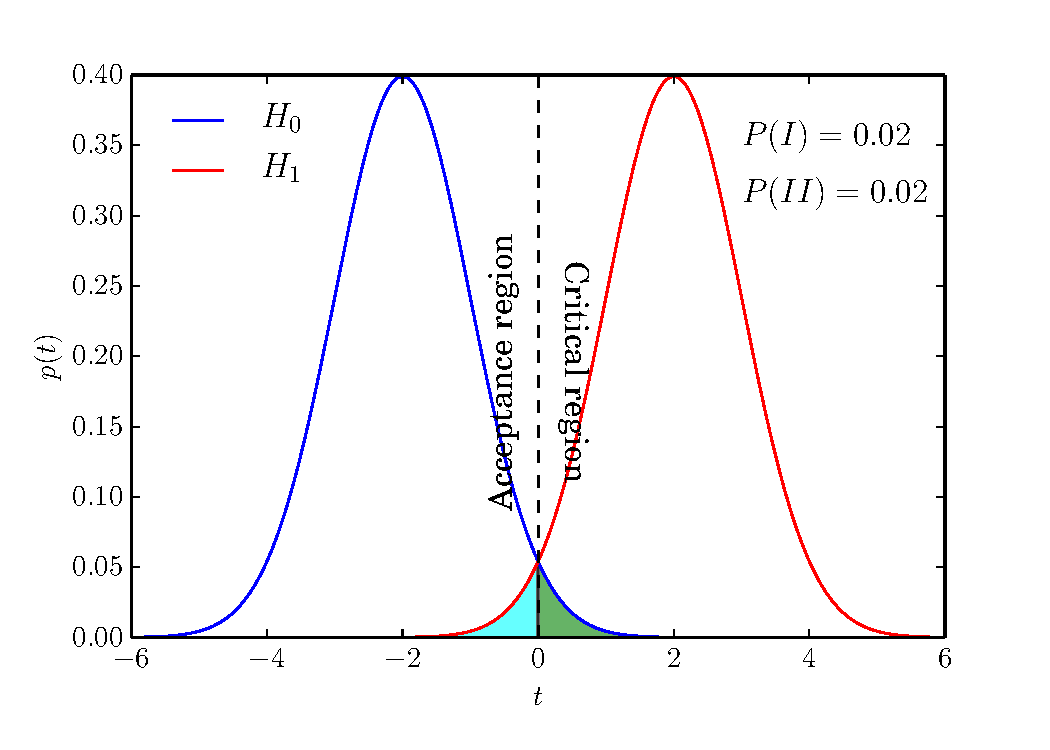
\includegraphics[keepaspectratio,width=\textwidth,height=200pt]{figures/hypothesis_test.pdf}
\end{column}
\end{columns}

\end{frame}

\begin{frame}

\frametitle{Hypothesis tests: example}
\label{hypothesistests:example}

\begin{columns}
    \begin{column}{0.3\textwidth}

If we define our \textbf{critical region} for $t$ (i.e. where we \emph{reject} $H_0$) as $t>0$ (so the \emph{acceptance
region} is $t\le0$) then we have:

\begin{itemize}
\item $p(I) = 0.02$

\item $p(II) = 0.02$

\item $\text{power} = 0.98$

\end{itemize}

\end{column}
    \begin{column}{0.7\textwidth}

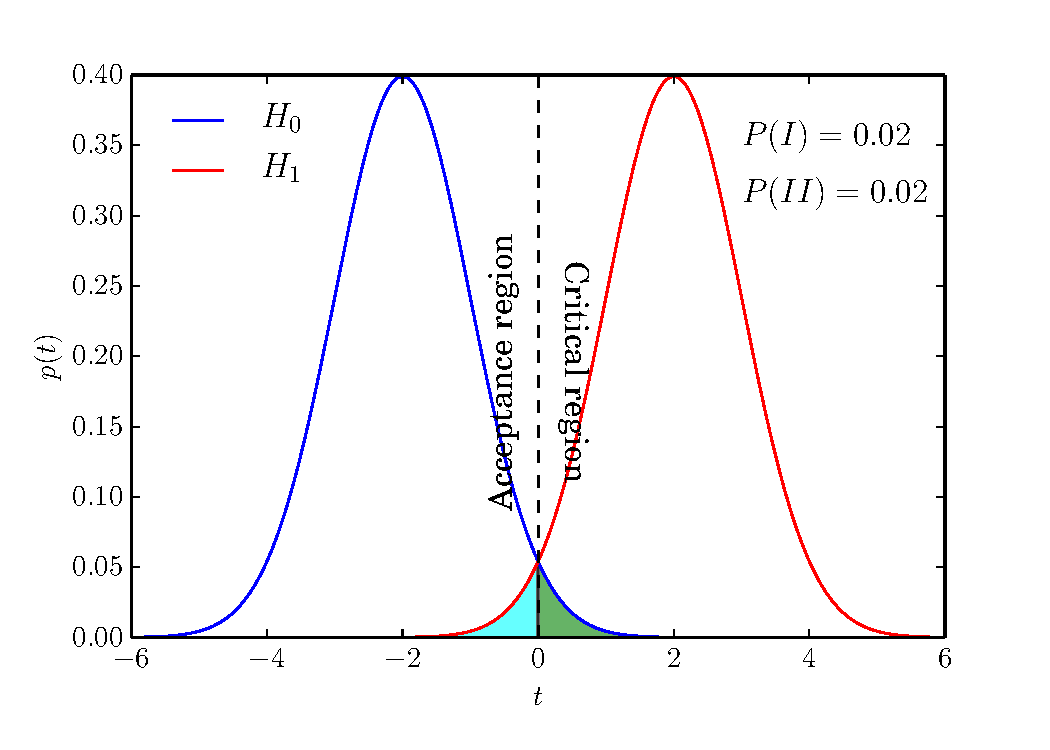
\includegraphics[keepaspectratio,width=\textwidth,height=200pt]{figures/hypothesis_test.pdf}
\end{column}
\end{columns}

\end{frame}

\begin{frame}

\frametitle{Hypothesis tests: significance}
\label{hypothesistests:significance}

The \textbf{level of significance} of a hypothesis test is the maximum probability of incurring a \emph{type I}
error that we are willing to risk. Commonly adopted levels are 5\% or 1\%.

If using 5\% then the \emph{critical region} is chosen so that $P(I) \le 0.05$. If the test statistic \emph{is}
within the critical region then we could say:

\begin{itemize}
\item the null hypothesis is rejected at the 5\% level, or

\item our rejecting of the null hypothesis is significant at the 5\% level, or

\item we are `95\% confident' we have made the correct decision in rejecting the null hypothesis

\end{itemize}

\end{frame}

\begin{frame}

\frametitle{Hypothesis tests: significance}
\label{hypothesistests:significance}

This is saying: \emph{if} the null hypothesis \emph{is} true and we repeat our experiment a large number of times
then we expect (by chance) the value of $t$ to lie within the critical region in no more than 5\% of them.

The choice of critical region and level of significance to assign is subjective. Ideally if the distributions
of $t$ for the two hypotheses have very little overlap (i.e. when signals are quite strong) one can be
stringent in setting the critical region so that $P(I)$ is very small, whilst only modestly increasing $P(II)$.
But, often that is not the case.

\end{frame}

\begin{frame}

\frametitle{Hypothesis tests: significance}
\label{hypothesistests:significance}

% New slide 

\begin{figure}[htbp]
\centering
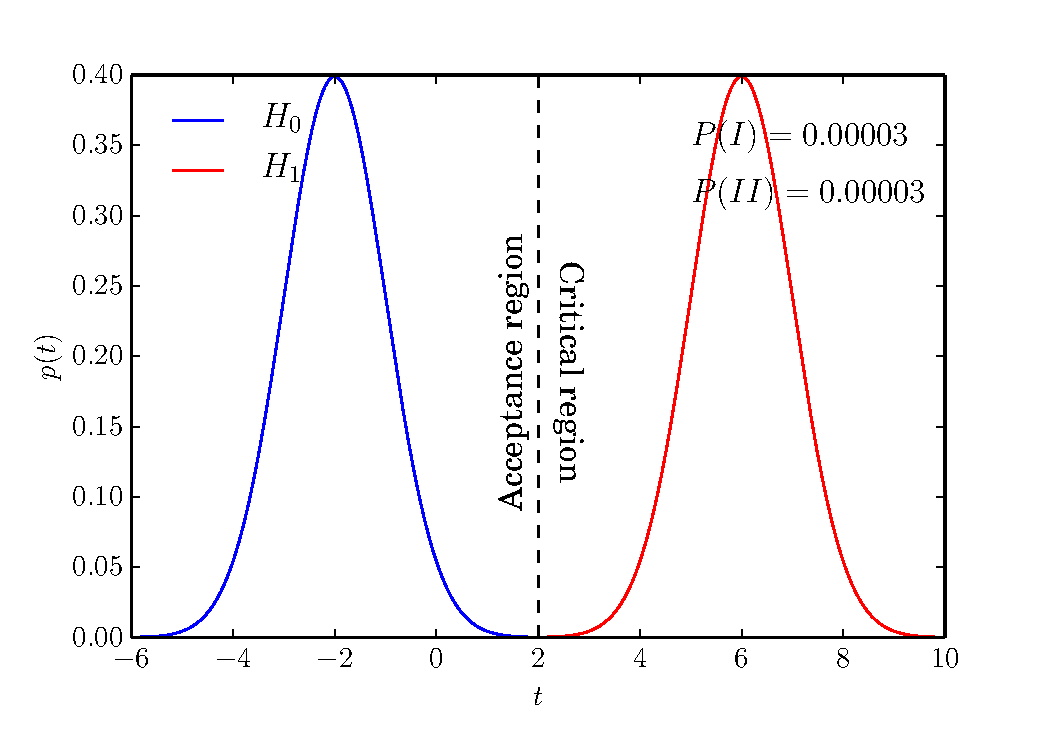
\includegraphics[keepaspectratio,width=\textwidth,height=210pt]{figures/hypothesis_test_2.pdf}
\label{hypothesis_test_2}
\end{figure}

\end{frame}

\begin{frame}

\frametitle{Simple hypothesis test example}
\label{simplehypothesistestexample}

Null hypothesis: \emph{sampled data are drawn from a normal pdf $N(\mu, \sigma^2)$ with with $\mu_{\rm model}$
and variance $\sigma^2$}. We want to \textbf{test} this null hypothesis (NH): are our data consistent with it?

Let's take some data, assuming a known variance and mean of their pdf, where:

\begin{itemize}
\item measured data: $\{x_i: i=1,\ldots,10\}$ and $\sum_{i=1}^{10}x_i = 47.8$, so the observed sample mean
$\hat{\mu}_{\rm obs} = 4.78$.

\item null hypothesis is that $x\sim N(\mu_{\rm model}, \sigma^2)$ where $\mu_{\rm model} =4$ and $\sigma=2$.

\end{itemize}

Under the null hypothesis the sample mean, $\hat{\mu}_{\rm model} \sim N(4, 2^2/10)$
(i.e. $\sigma_{\hat{\mu}} = \sigma^2/n = 2^2/10 = 0.4$). [Note: $x \sim N(\mu, \sigma^2)$
means $x$ \emph{is drawn from} $N$].

\end{frame}

\begin{frame}

\frametitle{Simple hypothesis test example}
\label{simplehypothesistestexample}

We can transform to a \emph{standard normal variable}, so under the NH:
\[
Z = \left( \frac{\hat{\mu}_{\rm obs}-\hat{\mu}_{\rm model}}{\sigma_{\hat{\mu}}}\right) \sim N(0,1).
\]
From our measured data:
\[
Z_{\rm obs} = \frac{4.78-4}{\sqrt{0.4}} = 1.233.
\]
So, \emph{if} NH is true, how probable is it that we would obtain a value of $Z_{\rm obs}$ as large as this, or larger?

We call this probability the \textbf{\color{red}p-value}. 

\end{frame}

\begin{frame}

\frametitle{Simple hypothesis test example}
\label{simplehypothesistestexample}

\[
p\text{-value} = \text{Prob}(|Z| \ge |Z_{\rm obs}|) = 1 - \int_{-Z_{\rm obs}}^{Z_{\rm obs}} \frac{1}{\sqrt{2\pi}}\exp{\left( -\frac{Z^2}{2}\right)} {\rm d}Z
\]

\begin{figure}[htbp]
\centering
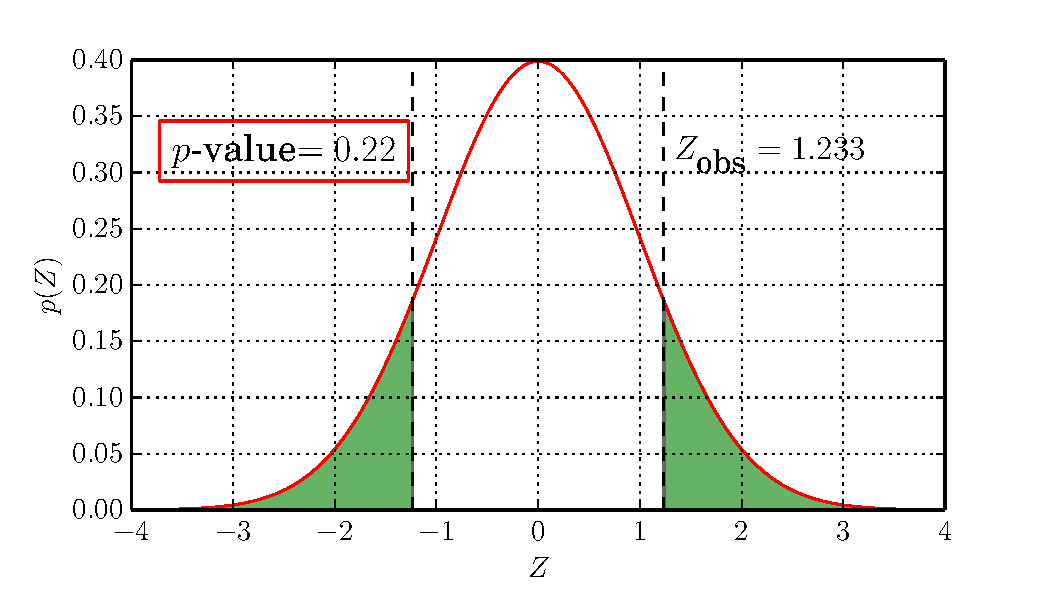
\includegraphics[keepaspectratio,width=\textwidth,height=155pt]{figures/pvalue.pdf}
\label{pvalue}
\end{figure}

\end{frame}

\begin{frame}

\frametitle{Simple hypothesis test example}
\label{simplehypothesistestexample}

In this case the p-value is 0.2176. The \emph{smaller} the p-value, the less credible is the null hypothesis.

Note: the p-value can be calculated using
\[
p\text{-value} = 1 - {\rm erf}(Z_{\rm obs}/\sqrt{2}),
\]
where ${\rm erf}$ is the \emph{error function}\footnote{The error function is available in e.g Matlab as \texttt{erf} and in python in \texttt{scipy.special.erf}.}
${\rm erf}(x) = \frac{2}{\sqrt{\pi}}\int_{0}^{x} e^{-y^2} {\rm d}y$.

This is a \emph{two-tailed} test, but the \emph{one-tailed} test could be used when appropriate for statistics with other sampling distributions.

\end{frame}

\begin{frame}

\frametitle{Simple hypothesis test example}
\label{simplehypothesistestexample}

\textbf{What if we \emph{don't} assume that $\sigma^2$ is known?}

Provided $n \ge 2$ we can estimate it from our observed data. We again form the statistic
\[
t_{\rm obs} = \left(\frac{\hat{\mu}_{\rm obs}-\hat{\mu}_{\rm model}}{\sigma_{\hat{\mu}}}\right),
\]
but now the variance on the sample mean is
\[
\sigma^2_{\hat{\mu}} = \frac{1}{n}\redub{\frac{1}{(n-1)}\sum_{i=1}^n (x_i - \hat{\mu}_{\rm obs})^2}_{\mathclap{\text{sample variance}}}
\]
However, unlike $Z_{\rm obs}$ previously, $t_{\rm obs}$ no longer has a normal distribution.

\end{frame}

\begin{frame}

\frametitle{Simple hypothesis test example}
\label{simplehypothesistestexample}

$t_{\rm obs}$ instead has a pdf known as the \textbf{Student's $t$-distribution}
\[
p(t) = \frac{\Gamma\left(\frac{\nu+1}{2}\right)}{\sqrt{\nu\pi}\Gamma\left(\frac{\nu}{2}\right)}\left(1+\frac{t^2}{\nu} \right)^{-\frac{\nu+1}{2}},
\]
where $\nu = n-1$ is the \textbf{number of degrees of freedom} and $\Gamma(\nu) = \int_0^{\infty}x^{\nu-1}e^{-x}{\rm d}x$.

For small $n$ (and therefore $\nu$) the Students's $t$-distribution has more extended tails than a
normal, but as $n \rightarrow \infty$ the distribution tends to $N(0,1)$.

\end{frame}

\begin{frame}

\frametitle{Simple hypothesis test example}
\label{simplehypothesistestexample}

\begin{figure}[htbp]
\centering
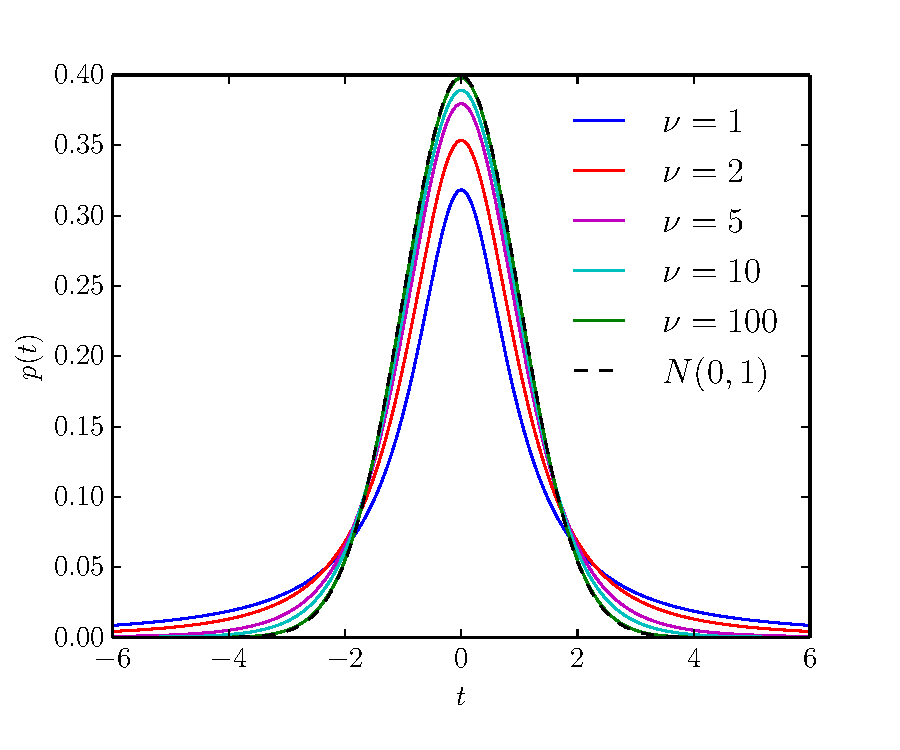
\includegraphics[keepaspectratio,width=\textwidth,height=210pt]{figures/studentst.pdf}
\label{studentst}
\end{figure}

\end{frame}

\begin{frame}

\frametitle{Goodness of Fit}
\label{goodnessoffit}

\begin{columns}
\begin{column}{0.35\textwidth}

As well as estimating parameters we might also want to ask how good our model was
(e.g. a straight line) in the first place. Given some data we can always obtain a best fit line, but it still
might be a very poor fit to the data.
\end{column}
\begin{column}{0.65\textwidth}
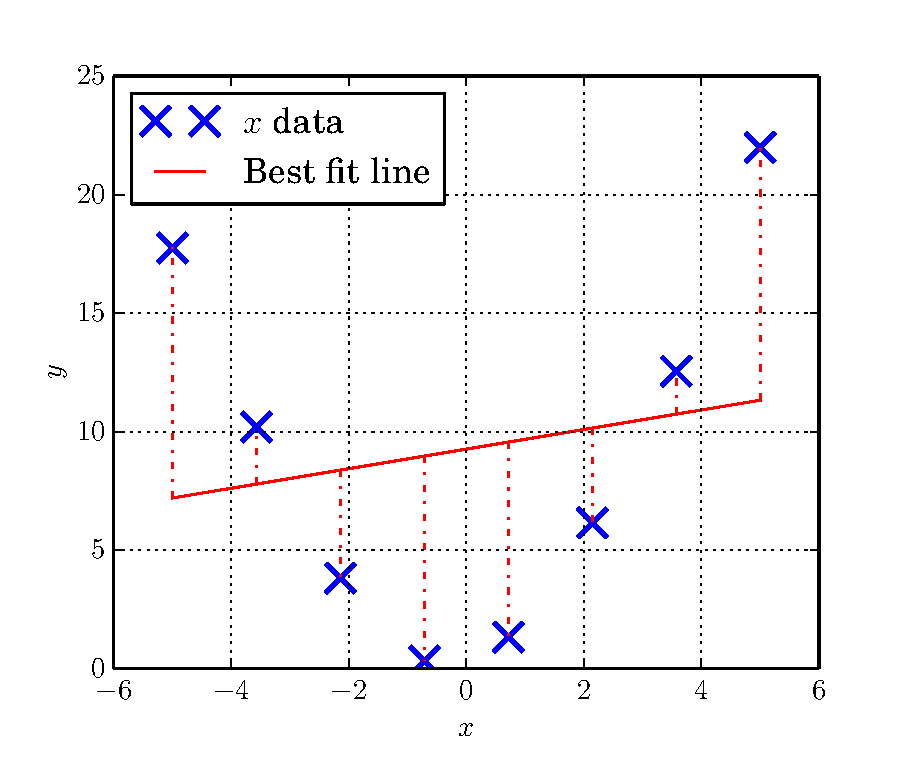
\includegraphics[keepaspectratio,width=\textwidth,height=210pt]{figures/quadratic_data.pdf}
\end{column}
\end{columns}

\end{frame}

\begin{frame}

\frametitle{Goodness of fit}
\label{goodnessoffit}

Answering how good our model is is tantamount to asking whether the residuals of the data are actually
drawn from their assumed distribution, i.e. a pdf with zero mean and a particular variance $\sigma^2$.

Suppose we have some true model $m_{\rm true}$ in the data $y$. The true residuals are given by
\[
\epsilon_i = y_i - m_{{\rm true},i},
\]
but unless $m_{\rm true}$ is already known these residuals are, in fact, \emph{unknown}. We only have our
`best fit' model (e.g. through least squares) $\hat{m}_{\rm LS}$, so we \emph{estimate} the residuals as
\[
\hat{\epsilon}_i = y_i - \hat{m}_{{\rm LS},i}.
\]

\end{frame}

\begin{frame}

\frametitle{Goodness of fit}
\label{goodnessoffit}

A goodness of fit test is an example of a simple hypothesis test. The basic ideas of a goodness-of-fit test are:

\begin{itemize}
\item choose a \textbf{null hypothesis}, where in this case a null hypothesis is defined as the statement being tested in our goodness of fit test\footnote{Often a null hypothesis is the statement that there is `no effect' present (e.g. the sampled
data are consistant with random noise, with a specified distribution, rather than contain a signal).}, for which we can evaluate a confidence level for its validity

\item select a suitable statistic that can be computed from the data and has a predictable distribution\footnote{the distribution we could expect to obtain under an infinite number of repeats of the data.}, e.g. a normal distribution.

\end{itemize}

\end{frame}

\begin{frame}

\frametitle{Goodness of fit: $\chi^2$ test}
\label{goodnessoffit:chi2test}

A commonly used goodness-of-fit test for model fitting is the $\chi^2$ statistic, given by
\[
\chi^2 = \sum_{i=1}^n \frac{\hat{\epsilon}^2_i}{\sigma_i^2} = \sum_{i=1}^n\frac{(y_i-\hat{m}_i)^2}{\sigma_i^2}
\]
where $y$ is the observed data, $\hat{m}$ is the `best fit' model (from e.g. the LS fit) and $\hat{\epsilon} = y_i-\hat{m}_i$ are the estimated residuals.

In this case, unless we know $\sigma_i$ \emph{a priori}, we can say nothing about the goodness of fit of our model. But,
if the residuals are distributed as $N(0, \sigma_i^2)$, then the $\chi^2$ statistic has a pdf given by
\[
p_{\nu}(\chi^2) = \frac{1}{2^{\frac{\nu}{2}}\Gamma\left(\frac{\nu}{2}\right)}\left(\chi^2\right)^{\frac{\nu}{2}-1}e^{-\chi^2/2}
\]

\end{frame}

\begin{frame}

\frametitle{Goodness of fit: $\chi^2$ test}
\label{goodnessoffit:chi2test}

\begin{columns}
    \begin{column}{0.25\textwidth}

Here $\nu$ is the number of \textbf{degrees of freedom} of the pdf, and the pdf has a mean of $\nu$ and variance of $2\nu$. As $\nu \rightarrow \infty$ the pdf tends to a normal pdf.
\end{column}
    \begin{column}{0.75\textwidth}
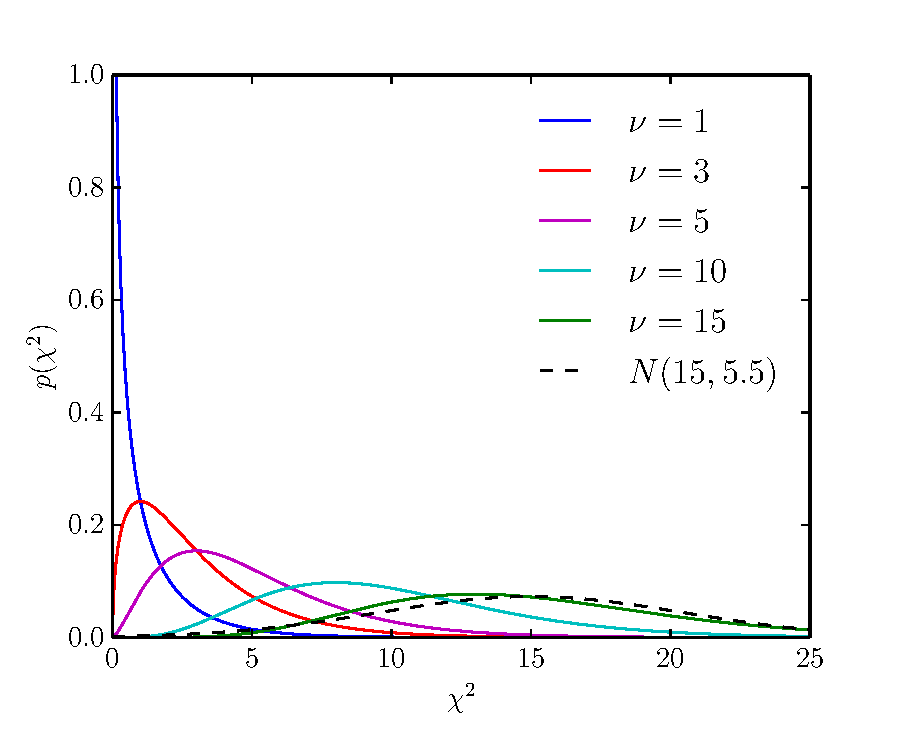
\includegraphics[keepaspectratio,width=\textwidth,height=200pt]{figures/chisquared.pdf}
\end{column}
\end{columns}

\end{frame}

\begin{frame}

\frametitle{Goodness of fit: $\chi^2$ test example}
\label{goodnessoffit:chi2testexample}

\begin{columns}
    \begin{column}{0.35\textwidth}

We have some power spectral density data, with a measurement error on each point $\sim N(0, 6.9^2)$.
Our \textbf{null hypothesis} is: \emph{the spectrum is constant, or flat, over all frequencies (i.e. there
are no spectral lines)}. We assume the residuals are iid and $\epsilon \sim N(0, \sigma^2)$.
\end{column}
    \begin{column}{0.65\textwidth}
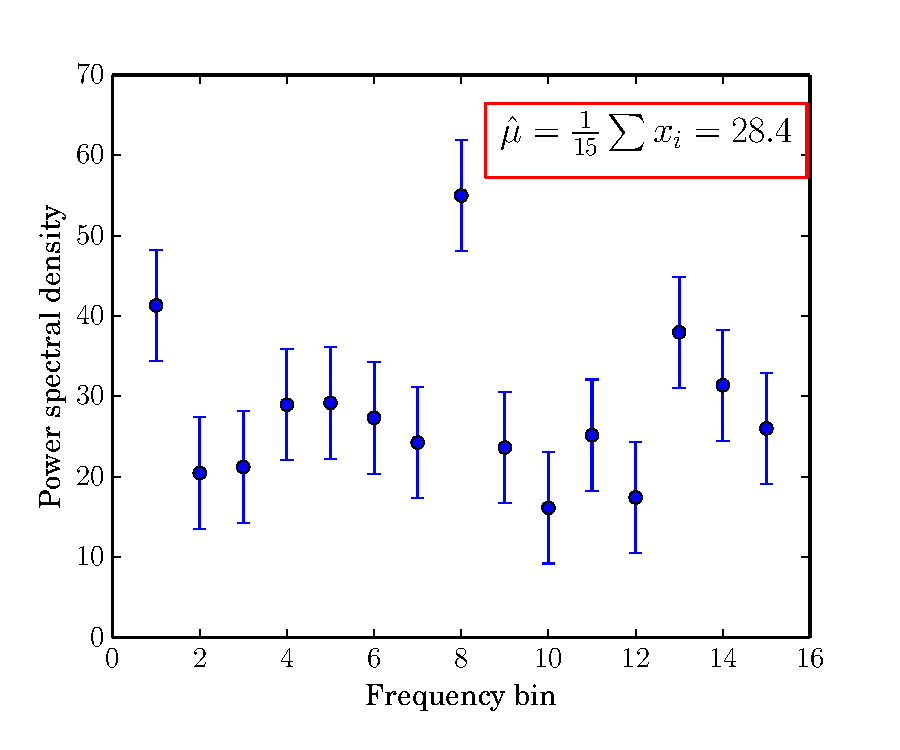
\includegraphics[keepaspectratio,width=\textwidth,height=200pt]{figures/chisquared_data.pdf}
\end{column}
\end{columns}

\end{frame}

\begin{frame}

\frametitle{Goodness of fit: $\chi^2$ test example}
\label{goodnessoffit:chi2testexample}

\[
\chi^2 = \sum_{i=1}^{n} \frac{(x_i - \hat{\mu})^2}{\sigma^2} = \sum_{i=1}^{15} \frac{(x_i-28.4)^2}{6.9^2} = 28.4
\]
\[
p_{\nu=(n-1)=14}(\chi^2) = p_{14}(28.4) = 29.6.
\]
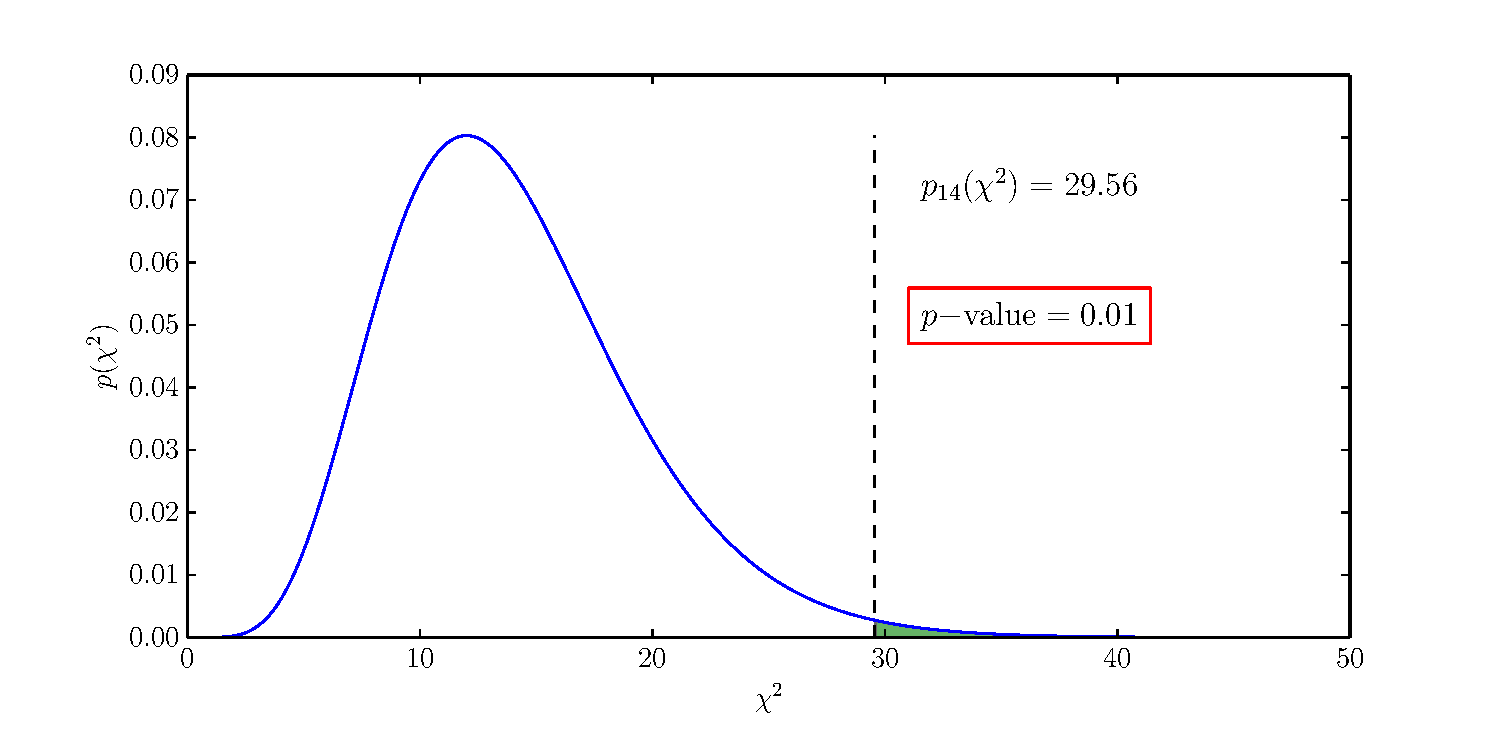
\includegraphics[keepaspectratio,width=\textwidth,height=170pt]{figures/chisquared_pdf.pdf}

\end{frame}

\begin{frame}

\frametitle{Goodness of fit: $\chi^2$ test example}
\label{goodnessoffit:chi2testexample}

So, \emph{if} the null hypothesis is true, how probable is it that we would measure as large, or larger, a
value of $\chi^2$?

We can again calculate a \textbf{p-value}, where this time is it given by
\begin{align*}
p\text{-value} &= 1 - P(\chi^2_{\rm obs} \ge \chi^2(\nu=14)), \\
&= 1-\int_0^{\chi^2_{\rm obs}} p_0 x^{\frac{\nu}{2}-1}e^{-x/2} {\rm d}x = 0.01,
\end{align*}
where $p_0 = 1/(2^{\nu/2}\Gamma(\nu/2))$.

\end{frame}

\begin{frame}

\frametitle{Goodness of fit: $\chi^2$ test example}
\label{goodnessoffit:chi2testexample}

What does this p-value mean?

\emph{If the spectrum really is flat, and we repeatedly obtained spectra of the same length under the same
conditions, then only 1\% of the $\chi^2$ values derived from these sets would be expected to be greater
than our one actual measured value of 29.6.}

I.e. if we obtain a very small p-value (e.g. a few percent?) we can interpret this as providing \emph{little support}
for the null hypothesis, which we may then choose to reject.

Ultimately this choice to reject a hypothesis is subjective, but the $\chi^2$ test can help in the decision.

\end{frame}

\begin{frame}

\frametitle{Goodness of fit: Kolmogorov-Smirnov test}
\label{goodnessoffit:kolmogorov-smirnovtest}

The \textbf{Kolmogorov-Smirnov test} (KS test) is a useful way to test the null hypothesis that a random sample
is drawn from a particular underlying pdf\footnote{The two sample KS test can also be used to compare whether two random samples are drawn
from the same underlying pdf $D_{m,n} = \text{max}\left|S_m(x) - S_n(x)\right|$.}, $p(x)$, with a known cdf $P(x)$.

If the iid sample $\{x_1,\ldots,x_n\}$ is arranged in ascending order, the sample cdf, $S_n(x)$, is
\[
S_n(x) = 
\begin{cases}
0, & \text{if } x < x_1 \\
\frac{i}{n}, & \text{if } x_i \le x < x_{i+1},~\text{for }1 \le i \le n-1 \\
1, & \text{if } x \ge x_n,
\end{cases}
\]
then the KS test statistic is defined as: $D_n = \text{max}\left|P(x) - S_n(x)\right|$.

\end{frame}

\begin{frame}

\frametitle{Goodness of fit: Kolmogorov-Smirnov test}
\label{goodnessoffit:kolmogorov-smirnovtest}

The distribution of $D_n$ under the null hypothesis is independent of the actual form of $P(x)$. Critical values
for the Kolmogorov distribution can be found online and associated p-values calculated.

The KS test for the case that the underlying pdf is normal is often called the \emph{Lilliefors test}.

The KS test is an example of a \textbf{nonparametric} test as there are minimum assumptions of a parametric form
of $p(x)$. However, this means its \textbf{power} is often lower than for other parametric tests, i.e. there is a
higher chance of false acceptance of the null hypothesis.

\end{frame}

\begin{frame}

\frametitle{Goodness of fit: Kolmogorov-Smirnov test}
\label{goodnessoffit:kolmogorov-smirnovtest}

\begin{columns}
    \begin{column}{0.3\textwidth}

We have a random sample of $30$ points $x \sim N(0,1)$ compared to a null hypothesis that $p(x) = N(0,1)$.
\end{column}
    \begin{column}{0.7\textwidth}
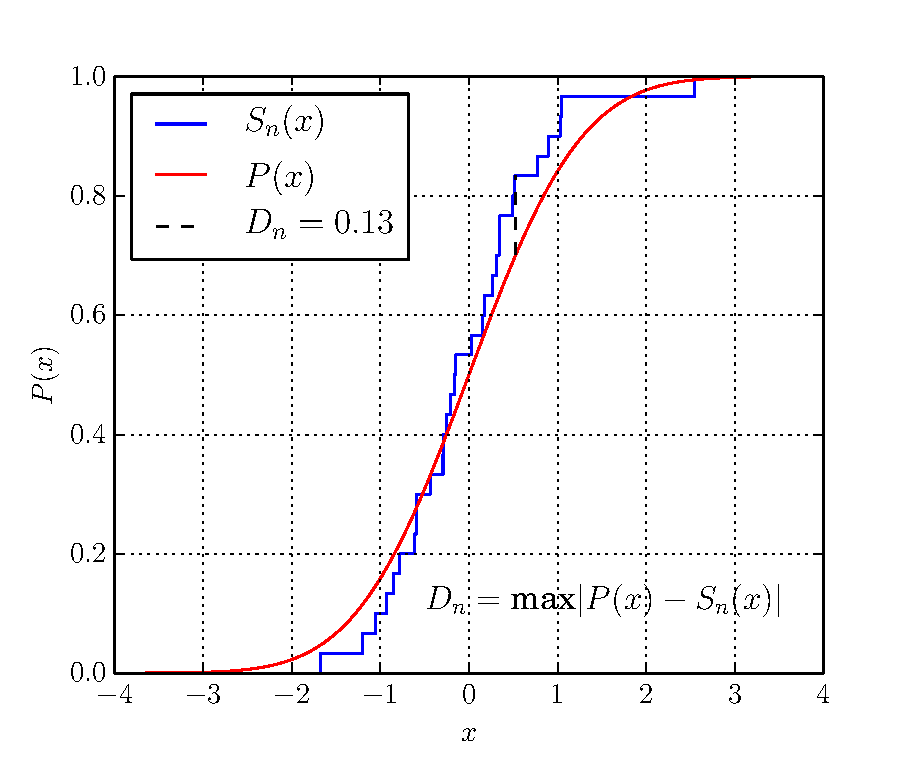
\includegraphics[keepaspectratio,width=\textwidth,height=210pt]{figures/kstest.pdf}
\end{column}
\end{columns}

\end{frame}

\begin{frame}

\frametitle{Goodness of fit: likelihood ratio test}
\label{goodnessoffit:likelihoodratiotest}

A simple test of the goodness of fit of two competing hypotheses, $H_0$ and $H_1$, defined by parameters $\theta_0$ and
$\theta_1$ respectively, is to form the likelihood ratio\footnote{Unlike the Bayesian odds ratio discussed in Part 3 this does not take into account any Occam factor} (generally using the maximum likehood
estimators $\hat{\theta}_0$ and $\hat{\theta}_1$)
\[
\Lambda(d) = \frac{L(\hat{\theta}_0)}{L(\hat{\theta}_1)}
\]
As with the other statistics we need to know the pdf of $\Lambda(d)$ to define critical regions for accessing
acceptance\slash rejection of hypotheses.

\end{frame}

\begin{frame}

\frametitle{Goodness of fit: likelihood ratio test}
\label{goodnessoffit:likelihoodratiotest}

Additional one could use the log-likelihood ratio test:
\[
D = -2\ln{\left(\frac{L(\hat{\theta}_0)}{L(\hat{\theta}_1)} \right)} = 2\left(\ln{L(\hat{\theta}_1)} - \ln{L(\hat{\theta}_0)}\right)
\]
The pdf of the test statistic $D$ is approximately a $\chi^2$-distribution with $\nu = (n_1-n_0)$ degrees
of freedom, where $n_1$ and $n_0$ are the number of free parameters for $H_0$ and $H_1$ respectively.

This type of statistic is common in gravitational wave data analysis, e.g. the $\mathcal{F}$-statistic ~\citep{JKS}
used in continuous wave searches.

\end{frame}

\begin{frame}

\frametitle{Goodness of fit: likelihood ratio test}
\label{goodnessoffit:likelihoodratiotest}

A simple example is:

\begin{itemize}
\item $H_0$: the data, $d$, consists of Gaussian noise with known $\sigma^2$, but an unknown mean $\mu$

\item $H_1$: the data, consists of Gaussian noise with known $\sigma^2$ and a mean of zero.

\end{itemize}

The best estimate of $\mu$ is just the sample mean $\hat{\mu}$, so using a Gaussian likelihood function we have
\[
\Lambda = \frac{ \cancel{(2\pi \sigma^2)^{-n/2}} \exp{\left(-\sum_{i=1}^n \frac{(d_i-\hat{\mu})^2}{2\sigma^2} \right)} }{ \cancel{(2\pi \sigma^2)^{-n/2}} \exp{\left(-\sum_{i=1}^n \frac{d_i^2}{2\sigma^2} \right)} } =
\exp{\left( -\sum_{i=1}^n \frac{\hat{\mu}^2 - 2d_i\hat{\mu}}{2\sigma^2} \right)}
\]
and
\[
D = \frac{\hat{\mu}\sum_{i=1}^n (\hat{\mu} - 2 d_i)}{\sigma^2} = -\frac{\sum_{i=1}^n \hat{\mu} d_i}{\sigma^2} = -\frac{\left(\sum_{i=1}^n d_i\right)^2}{n\sigma^2}
\]

\end{frame}

\begin{frame}

\frametitle{Goodness of fit: others tests}
\label{goodnessoffit:otherstests}

Other common tests are:

\begin{itemize}
\item $F$-test - test where two random samples have the same variance using the $f$-statistic defined
as the ratio of the variances

\item sample correlation coefficient - test whether two variables are statistically independent

\end{itemize}

\end{frame}

\begin{frame}

\frametitle{Confidence intervals}
\label{confidenceintervals}

In parameter estimation we had a point \textbf{estimator} for a parameter i.e. a single number, $\hat{\theta}$,
which we associate with the \emph{true} (but unknown) value of the parameter $\theta$. But, we might want to assess
the likely \emph{range} of the true values of $\theta$. To do this we can define \textbf{confidence intervals}. 

If we know (or assume) the pdf of the estimator $p(\hat{\theta})$ (e.g. a normal
$N(\hat{\theta},\sigma^2_{\hat{\theta}})$) then we can define a confidence interval for $\theta$
$[\theta_a,\theta_b]$ as
\[
X = \text{Prob}(\theta_a \le \theta \le \theta_b) = \int_{\theta_a}^{\theta_b} p(\hat{\theta}) {\rm d}\hat{\theta}.
\]

\end{frame}

\begin{frame}

\frametitle{Confidence intervals}
\label{confidenceintervals}

\[
X = \text{Prob}(\theta_a \le \theta \le \theta_b) = \int_{\theta_a}^{\theta_b} p(\hat{\theta}) {\rm d}\hat{\theta},
\]
where, e.g. $X=0.95$ would give the \textbf{95\% confidence interval} and $[\theta_a, \theta_b]$ would be the
\textbf{95\% confidence limits}.

Note that $\theta_a$ and $\theta_b$ are not unique, but you could define them
to represent the \emph{shortest interval} or to be symmetric about $\hat{\theta}$.

If $p(\hat{\theta})$ is a normal distribution then
\[
\text{Prob}\left(\hat{\theta}-1.96\sqrt{\sigma^2_{\hat{\theta}}} \le \theta \le \hat{\theta}+1.96\sqrt{\sigma^2_{\hat{\theta}}}\right) = 0.95
\]

\end{frame}

\begin{frame}

\frametitle{Confidence intervals: interpretation}
\label{confidenceintervals:interpretation}

For a single random sample (experiment) $\hat{\theta}$ is a unique number, so the probability that the
true $\theta$ lies in a chosen confidence interval is either zero or one.

To interpret confidence intervals one needs to think in terms of repeating the experiment\slash observation
that produced the random sample a large number of times. For each a different value of $\hat{\theta}$
would be produced, and hence also different confidence limits for $\theta$, for the \emph{same} fixed (but
unknown) $\theta$.

Thus confidence intervals, for e.g. $X=0.95\%$, mean that we would expect $\theta$ to lie within their range
in 95\% of a large number of experiments. Thus, we are \textbf{95\% confident} that $\theta$ lies within the interval
given from our actual observed value $\hat{\theta}$.

% Bibliography slide 

\end{frame}

\begin{frame}

\frametitle{Bibliography}
\label{bibliography}


\bibliographystyle{unsrt}
\bibliography{stats_part02}


\end{frame}

\mode<all>
\input{mmd-beamer-footer}

\end{document}\mode*

